\begin{enumerate}[label=\thesubsection.\arabic*,ref=\thesubsection.\theenumi]
\item Find the shortest distance between the lines
\begin{align}
	\frac{x+1}{7}&=\frac{y+1}{-6}=\frac{z+1}{1} \text{ and}
	\\
	\frac{x-3}{1}&=\frac{y-5}{-2}=\frac{z-7}{1}
\end{align}
    \solution
		%\begin{enumerate}[label=\arabic*.,ref=\theenumi]
\begin{enumerate}[label=\thesubsection.\arabic*.,ref=\thesubsection.\theenumi]
	\item The lines
\begin{align}
\begin{split}
	L_1: \quad   \vec{x} &=\vec{A}+ \kappa_1\vec{m_1}
	\\
L_2: \quad        
	\vec{x} &= \vec{B}  + \kappa_2\vec{m_2} 
\end{split}
	    \label{eq:chapters/12/11/2/16/lsq/L1L2}
\end{align}
will intersect if 
\begin{align}
\vec{A}+ \kappa_1\vec{m_1}
= \vec{B}  + \kappa_2\vec{m_2} 
\\
\implies 
 \myvec{\vec{m_1} & \vec{m_2}}\myvec{\kappa_1\\-\kappa_2}
	 =\vec{B}-\vec{A}
 \\
	\implies \rank\myvec{\vec{M}  
	& \vec{B}-\vec{A}} = 2 
	    \label{eq:chapters/12/11/2/16/lsq/rank}
\end{align}
where
\begin{align}
	\vec{M} = 
	\myvec{\vec{m_1} & \vec{m_2}} 
\end{align}
\item If $L_1, L_2$, do not intersect, let 
\begin{align}
\begin{split}
	\vec{x}_1 &=\vec{A}+ \kappa_1\vec{m_1}
	\\
	\vec{x}_2 &= \vec{B}  + \kappa_2\vec{m_2} 
\end{split}
	    \label{eq:chapters/12/11/2/16/lsq/x1x2}
\end{align}
be points on 
$L_1, L_2$ respectively, that are closest to each other.
Then, 
	    from \eqref{eq:chapters/12/11/2/16/lsq/x1x2}
\begin{align}
\vec{x_1} - \vec{x_2} =
	 \vec{A}-\vec{B}+
 \myvec{\vec{m_1} & \vec{m_2}}\myvec{\kappa_1\\-\kappa_2}
	\label{eq:chapters/12/11/2/16/lsq/x-diff}
\end{align}
Also, 
    \begin{align}
	    \brak{\vec{x}_1 -\vec{x}_2}^\top\vec{m}_1
	    =
	    \brak{\vec{x}_1 -\vec{x}_2}^\top\vec{m}_2
	    =0
	    \\
	    \implies 
	    \brak{\vec{x}_1 -\vec{x}_2}^\top\myvec{\vec{m_1} & \vec{m_2}} = \vec{0}
	    \\
	    \text{or, }	    \vec{M}^\top\brak{\vec{x}_1 -\vec{x}_2} = \vec{0}
	    \\
	    \implies \vec{M}^\top
	    \brak{\vec{A}-\vec{B}}+
 \vec{M}^\top\vec{M}\myvec{\kappa_1\\-\kappa_2} = \vec{0}
	    \label{eq:chapters/12/11/2/16/lsq/m-orth}
    \end{align}
	    from 
	\eqref{eq:chapters/12/11/2/16/lsq/x-diff},
	yielding
    \begin{align}
	    \vec{M}^\top\vec{M}\myvec{\kappa_1\\-\kappa_2} = \vec{M}^\top\brak{\vec{B}-\vec{A}}
        \label{eq:chapters/12/11/2/16/lsq/vec-eqn}
    \end{align}
    This is known as the {\em least squares solution}.
	\item Perform the eigendecompositions 
    \begin{align}
	    \vec{MM}^\top &= \vec{U}\vec{D}_1\vec{U}^\top \label{eq:chapters/12/11/2/16/svd/decomp-1} \\
	    \vec{M}^\top\vec{M} &= \vec{V}\vec{D}_2\vec{V}^\top \label{eq:chapters/12/11/2/16/svd/decomp-2}
    \end{align}
	\item    The following expression is known as {\em singular value decomposition}
    \begin{align}
        \vec{M} = 
	\vec{U}\vec{\Sigma}\vec{V}^\top
        \label{eq:chapters/12/11/2/16/svd/M-svd}
    \end{align}
    where $\vec{\Sigma}$ is diagonal with
    entries obtained as in 
        \eqref{eq:chapters/12/11/2/16/svd/svd-params}.
 Substituting in 
        \eqref{eq:chapters/12/11/2/16/lsq/vec-eqn},
	\begin{align}
\vec{V}\vec{\Sigma}\vec{U}^\top\vec{U}\vec{\Sigma}\vec{V}^\top\bm{\kappa} &= \vec{V}\vec{\Sigma}\vec{U}^\top\brak{\vec{B}-\vec{A}} \\
\implies \vec{V}\vec{\Sigma}^2\vec{V}^\top\bm{\kappa} &= \vec{V}\vec{\Sigma}\vec{U}^\top\brak{\vec{B}-\vec{A}} \\
\implies \bm{\kappa} &= \brak{\vec{V}\vec{\Sigma}^2\vec{V}^\top}^{-1}\vec{V}\vec{\Sigma}\vec{U}^\top\brak{\vec{B}-\vec{A}} \\
\implies \bm{\kappa} &= \vec{V}\vec{\Sigma}^{-2}\vec{V}^\top\vec{V}\vec{\Sigma}\vec{U}^\top\brak{\vec{B}-\vec{A}} \\
\implies \bm{\kappa} &= \vec{V}\vec{\Sigma}^{-1}\vec{U}^\top\brak{\vec{B}-\vec{A}}
\label{eq:chapters/12/11/2/16/svd/kappa-sol}
\end{align}
    where $\vec{\Sigma}^{-1}$ is obtained by inverting the nonzero elements of
    $\vec{\Sigma}$. 
		\item 
	    From \eqref{eq:chapters/12/11/2/16/lsq/x1x2}, 
\begin{align}
	\vec{x}_1-\vec{x}_2 &= 
	\vec{A}+ \kappa_1\vec{m_1}
	 -\vec{B}  - \kappa_2\vec{m_2} 
	 \\
	 &=
	\vec{A} 
	 -\vec{B}  + \vec{M} 
	\bm{\kappa}
\end{align}
which, upon substitution from 
        \eqref{eq:chapters/12/11/2/16/svd/M-svd}
	yields
\begin{align}
	\vec{x}_1-\vec{x}_2 &= 
	\vec{A} 
	 -\vec{B}  + 
\vec{U}\vec{\Sigma}\vec{V}^\top
\vec{V}\vec{\Sigma}^{-1}\vec{U}^\top\brak{\vec{B}-\vec{A}}
\\
	&=
	\brak{	\vec{A} 
	 -\vec{B}}  \brak{\vec{I}- 
\vec{U}\vec{\Sigma}
	\vec{\Sigma}^{-1}\vec{U}^\top}
\end{align}
			Thus, 
    \begin{align}
	    \norm{\vec{x}_1-\vec{x}_2} = 
	\norm{\brak{	\vec{A} 
	 -\vec{B}}  \brak{\vec{I}- 
\vec{U}\vec{\Sigma}
	    \vec{\Sigma}^{-1}\vec{U}^\top}}
        \label{eq:chapters/12/11/2/16/svd/min-sol}
    \end{align}
\item Least squares solution
	\begin{lstlisting}
	codes/book/skew_least.py
\end{lstlisting}
\item Least squares using builtin SVD 
	\begin{lstlisting}
	codes/book/skew_builtin.py
\end{lstlisting}
\item Code linking eigenvalues and singular values
	\begin{lstlisting}
	codes/book/skew_svd.py
\end{lstlisting}
\end{enumerate}

    \item Find the shortest distance between the lines whose vector equations are
    \begin{align}
\begin{split}
	\vec{x} &= \myvec{1\\2\\3} + \kappa_1\myvec{1\\-3\\2}
	\\
	\vec{x} &= \myvec{4\\5\\6} + \kappa_2\myvec{2\\3\\1}
\end{split}
        \label{eq:chapters/12/11/2/16/L2/svd}
    \end{align}
    \solution
		%\begin{enumerate}[label=\arabic*.,ref=\theenumi]
\begin{enumerate}[label=\thesubsection.\arabic*.,ref=\thesubsection.\theenumi]
	\item The lines
\begin{align}
\begin{split}
	L_1: \quad   \vec{x} &=\vec{A}+ \kappa_1\vec{m_1}
	\\
L_2: \quad        
	\vec{x} &= \vec{B}  + \kappa_2\vec{m_2} 
\end{split}
	    \label{eq:chapters/12/11/2/16/lsq/L1L2}
\end{align}
will intersect if 
\begin{align}
\vec{A}+ \kappa_1\vec{m_1}
= \vec{B}  + \kappa_2\vec{m_2} 
\\
\implies 
 \myvec{\vec{m_1} & \vec{m_2}}\myvec{\kappa_1\\-\kappa_2}
	 =\vec{B}-\vec{A}
 \\
	\implies \rank\myvec{\vec{M}  
	& \vec{B}-\vec{A}} = 2 
	    \label{eq:chapters/12/11/2/16/lsq/rank}
\end{align}
where
\begin{align}
	\vec{M} = 
	\myvec{\vec{m_1} & \vec{m_2}} 
\end{align}
\item If $L_1, L_2$, do not intersect, let 
\begin{align}
\begin{split}
	\vec{x}_1 &=\vec{A}+ \kappa_1\vec{m_1}
	\\
	\vec{x}_2 &= \vec{B}  + \kappa_2\vec{m_2} 
\end{split}
	    \label{eq:chapters/12/11/2/16/lsq/x1x2}
\end{align}
be points on 
$L_1, L_2$ respectively, that are closest to each other.
Then, 
	    from \eqref{eq:chapters/12/11/2/16/lsq/x1x2}
\begin{align}
\vec{x_1} - \vec{x_2} =
	 \vec{A}-\vec{B}+
 \myvec{\vec{m_1} & \vec{m_2}}\myvec{\kappa_1\\-\kappa_2}
	\label{eq:chapters/12/11/2/16/lsq/x-diff}
\end{align}
Also, 
    \begin{align}
	    \brak{\vec{x}_1 -\vec{x}_2}^\top\vec{m}_1
	    =
	    \brak{\vec{x}_1 -\vec{x}_2}^\top\vec{m}_2
	    =0
	    \\
	    \implies 
	    \brak{\vec{x}_1 -\vec{x}_2}^\top\myvec{\vec{m_1} & \vec{m_2}} = \vec{0}
	    \\
	    \text{or, }	    \vec{M}^\top\brak{\vec{x}_1 -\vec{x}_2} = \vec{0}
	    \\
	    \implies \vec{M}^\top
	    \brak{\vec{A}-\vec{B}}+
 \vec{M}^\top\vec{M}\myvec{\kappa_1\\-\kappa_2} = \vec{0}
	    \label{eq:chapters/12/11/2/16/lsq/m-orth}
    \end{align}
	    from 
	\eqref{eq:chapters/12/11/2/16/lsq/x-diff},
	yielding
    \begin{align}
	    \vec{M}^\top\vec{M}\myvec{\kappa_1\\-\kappa_2} = \vec{M}^\top\brak{\vec{B}-\vec{A}}
        \label{eq:chapters/12/11/2/16/lsq/vec-eqn}
    \end{align}
    This is known as the {\em least squares solution}.
	\item Perform the eigendecompositions 
    \begin{align}
	    \vec{MM}^\top &= \vec{U}\vec{D}_1\vec{U}^\top \label{eq:chapters/12/11/2/16/svd/decomp-1} \\
	    \vec{M}^\top\vec{M} &= \vec{V}\vec{D}_2\vec{V}^\top \label{eq:chapters/12/11/2/16/svd/decomp-2}
    \end{align}
	\item    The following expression is known as {\em singular value decomposition}
    \begin{align}
        \vec{M} = 
	\vec{U}\vec{\Sigma}\vec{V}^\top
        \label{eq:chapters/12/11/2/16/svd/M-svd}
    \end{align}
    where $\vec{\Sigma}$ is diagonal with
    entries obtained as in 
        \eqref{eq:chapters/12/11/2/16/svd/svd-params}.
 Substituting in 
        \eqref{eq:chapters/12/11/2/16/lsq/vec-eqn},
	\begin{align}
\vec{V}\vec{\Sigma}\vec{U}^\top\vec{U}\vec{\Sigma}\vec{V}^\top\bm{\kappa} &= \vec{V}\vec{\Sigma}\vec{U}^\top\brak{\vec{B}-\vec{A}} \\
\implies \vec{V}\vec{\Sigma}^2\vec{V}^\top\bm{\kappa} &= \vec{V}\vec{\Sigma}\vec{U}^\top\brak{\vec{B}-\vec{A}} \\
\implies \bm{\kappa} &= \brak{\vec{V}\vec{\Sigma}^2\vec{V}^\top}^{-1}\vec{V}\vec{\Sigma}\vec{U}^\top\brak{\vec{B}-\vec{A}} \\
\implies \bm{\kappa} &= \vec{V}\vec{\Sigma}^{-2}\vec{V}^\top\vec{V}\vec{\Sigma}\vec{U}^\top\brak{\vec{B}-\vec{A}} \\
\implies \bm{\kappa} &= \vec{V}\vec{\Sigma}^{-1}\vec{U}^\top\brak{\vec{B}-\vec{A}}
\label{eq:chapters/12/11/2/16/svd/kappa-sol}
\end{align}
    where $\vec{\Sigma}^{-1}$ is obtained by inverting the nonzero elements of
    $\vec{\Sigma}$. 
		\item 
	    From \eqref{eq:chapters/12/11/2/16/lsq/x1x2}, 
\begin{align}
	\vec{x}_1-\vec{x}_2 &= 
	\vec{A}+ \kappa_1\vec{m_1}
	 -\vec{B}  - \kappa_2\vec{m_2} 
	 \\
	 &=
	\vec{A} 
	 -\vec{B}  + \vec{M} 
	\bm{\kappa}
\end{align}
which, upon substitution from 
        \eqref{eq:chapters/12/11/2/16/svd/M-svd}
	yields
\begin{align}
	\vec{x}_1-\vec{x}_2 &= 
	\vec{A} 
	 -\vec{B}  + 
\vec{U}\vec{\Sigma}\vec{V}^\top
\vec{V}\vec{\Sigma}^{-1}\vec{U}^\top\brak{\vec{B}-\vec{A}}
\\
	&=
	\brak{	\vec{A} 
	 -\vec{B}}  \brak{\vec{I}- 
\vec{U}\vec{\Sigma}
	\vec{\Sigma}^{-1}\vec{U}^\top}
\end{align}
			Thus, 
    \begin{align}
	    \norm{\vec{x}_1-\vec{x}_2} = 
	\norm{\brak{	\vec{A} 
	 -\vec{B}}  \brak{\vec{I}- 
\vec{U}\vec{\Sigma}
	    \vec{\Sigma}^{-1}\vec{U}^\top}}
        \label{eq:chapters/12/11/2/16/svd/min-sol}
    \end{align}
\item Least squares solution
	\begin{lstlisting}
	codes/book/skew_least.py
\end{lstlisting}
\item Least squares using builtin SVD 
	\begin{lstlisting}
	codes/book/skew_builtin.py
\end{lstlisting}
\item Code linking eigenvalues and singular values
	\begin{lstlisting}
	codes/book/skew_svd.py
\end{lstlisting}
\end{enumerate}

\item Find the shortest distance between the lines $l_1$ and $l_2$ whose vector equations are 
\begin{align}
	\overrightarrow{r} &= \hat{i}+\hat{j}+\kappa(2\hat{i}-\hat{j}+\hat{k}) \text{ and}
	\\
	\overrightarrow{r} &= 2\hat{i}+\hat{j}-\hat{k}+\mu(3\hat{i}-5\hat{j}+2\hat{k}).
\end{align}
    \solution
		\\ \solution 
\begin{align}
    \vec{A}-\vec{F}&=\myvec{1\\-1}-\myvec{\frac{-3}{2}\\\frac{5}{2}}
    =\myvec{\frac{5}{2}\\\frac{-7}{2}}
    \\
    \vec{E}-\vec{D}&=\myvec{-1\\-3}-\myvec{\frac{-7}{2}\\\frac{1}{2}}
    =\myvec{\frac{5}{2}\\\frac{-7}{2}}
    \\
	\implies	\vec{A}-\vec{F} &= \vec{E}-\vec{D}
\end{align}
See \figref{fig:Triangle-pgm}, 
\begin{figure}
\centering
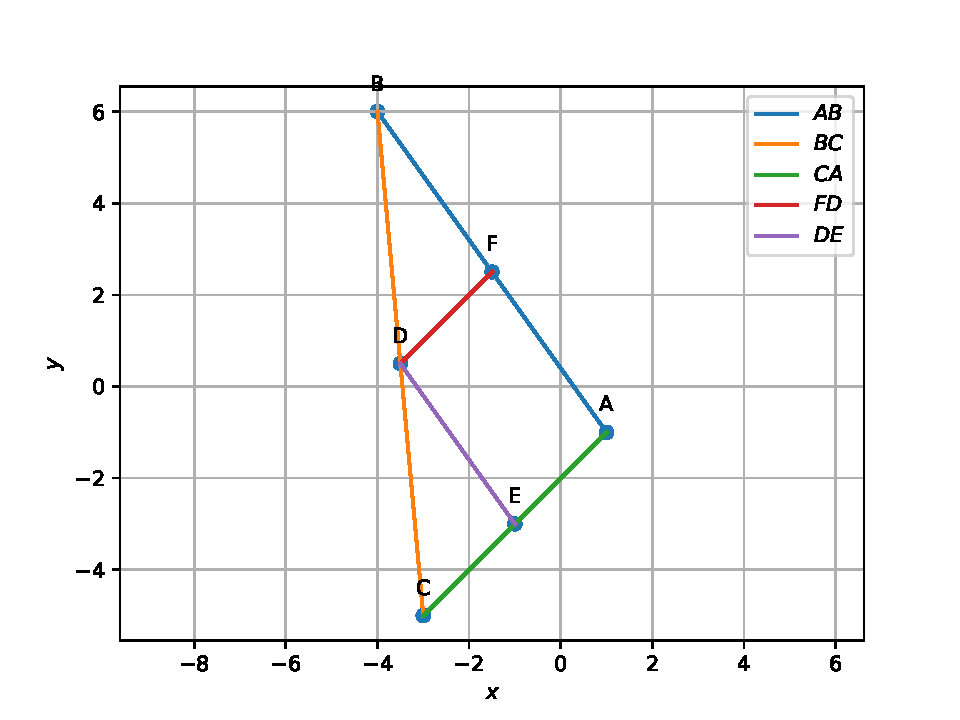
\includegraphics[width=0.75\columnwidth]{figs/triangle/pgm.pdf}
\caption{$AFDE$ forms a parallelogram in triangle ABC}
\label{fig:Triangle-pgm}
\end{figure}






















		%\begin{enumerate}[label=\thesubsection.\arabic*,ref=\thesubsection.\theenumi]
    \item Find the shortest distance between the lines whose vector equations are
    \begin{align}
        \vec{x} = \myvec{1\\2\\3} + \lambda_1\myvec{1\\-3\\2}
    \end{align}
    and
    \begin{align}
        \vec{x} = \myvec{4\\5\\6} + \lambda_2\myvec{2\\3\\1}
    \end{align}
    \solution
		\\ \solution 
\begin{align}
    \vec{A}-\vec{F}&=\myvec{1\\-1}-\myvec{\frac{-3}{2}\\\frac{5}{2}}
    =\myvec{\frac{5}{2}\\\frac{-7}{2}}
    \\
    \vec{E}-\vec{D}&=\myvec{-1\\-3}-\myvec{\frac{-7}{2}\\\frac{1}{2}}
    =\myvec{\frac{5}{2}\\\frac{-7}{2}}
    \\
	\implies	\vec{A}-\vec{F} &= \vec{E}-\vec{D}
\end{align}
See \figref{fig:Triangle-pgm}, 
\begin{figure}
\centering
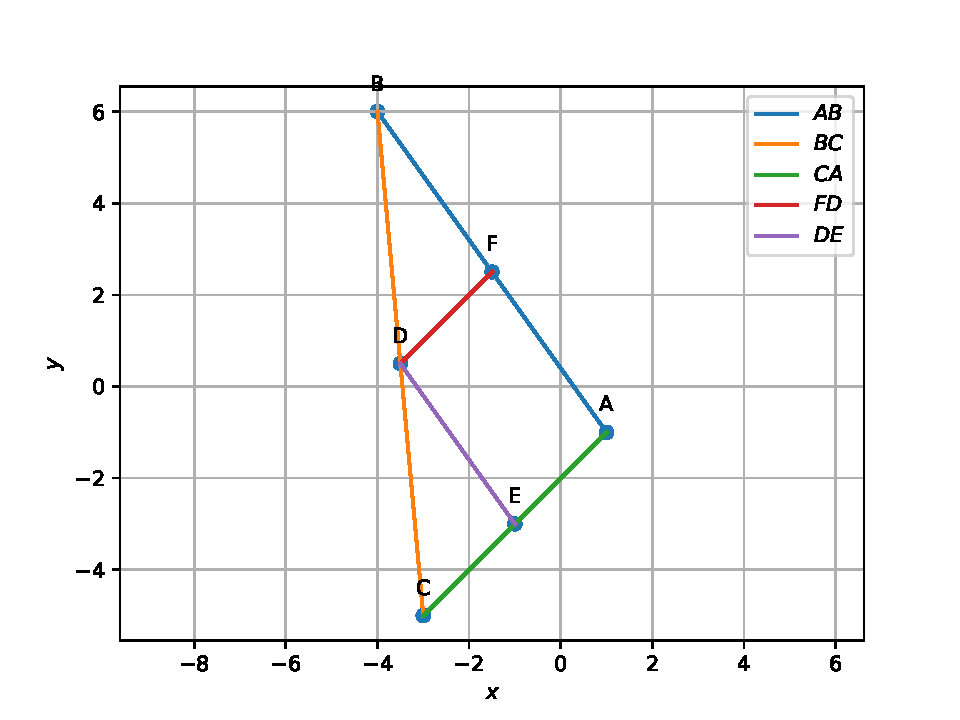
\includegraphics[width=0.75\columnwidth]{figs/triangle/pgm.pdf}
\caption{$AFDE$ forms a parallelogram in triangle ABC}
\label{fig:Triangle-pgm}
\end{figure}






















\item Find the shortest distance between the lines $l_1$ and $l_2$ whose vector equations are 
\begin{align}
	\overrightarrow{r} &= \hat{i}+\hat{j}+\lambda(2\hat{i}-\hat{j}+\hat{k}) \text{ and}
	\\
	\overrightarrow{r} &= 2\hat{i}+\hat{j}-\hat{k}+\mu(3\hat{i}-5\hat{j}+2\hat{k}).
\end{align}
    \solution
		\\ \solution 
\begin{align}
    \vec{A}-\vec{F}&=\myvec{1\\-1}-\myvec{\frac{-3}{2}\\\frac{5}{2}}
    =\myvec{\frac{5}{2}\\\frac{-7}{2}}
    \\
    \vec{E}-\vec{D}&=\myvec{-1\\-3}-\myvec{\frac{-7}{2}\\\frac{1}{2}}
    =\myvec{\frac{5}{2}\\\frac{-7}{2}}
    \\
	\implies	\vec{A}-\vec{F} &= \vec{E}-\vec{D}
\end{align}
See \figref{fig:Triangle-pgm}, 
\begin{figure}
\centering
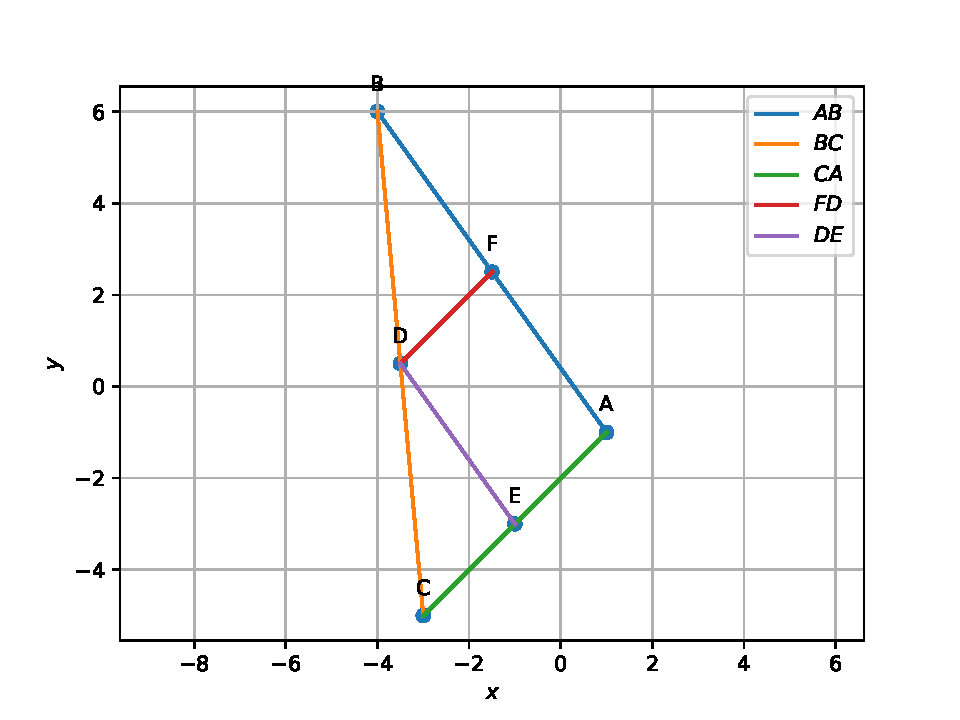
\includegraphics[width=0.75\columnwidth]{figs/triangle/pgm.pdf}
\caption{$AFDE$ forms a parallelogram in triangle ABC}
\label{fig:Triangle-pgm}
\end{figure}






















\item Find the shortest distance between the lines given by 
\begin{align}
	\overrightarrow{r}&=(8+3\lambda\hat{i}-(9+16\lambda)\hat{j}+(10+7\lambda)\hat{k} \text{ and} 
	\\
	\overrightarrow{r}&=15\hat{i}+29\hat{j}+5\hat{k}+\mu(3\hat{i}+8\hat{j}-5\hat{k}).
\end{align}
\item Find the shortest distance between the lines
\begin{align}
	\overrightarrow{r}&=(\hat{i}+2\hat{j}+\hat{k})+\lambda(\hat{i}-\hat{j}+\hat{k}) \text{ and} 
	\\
	\overrightarrow{r}&=2\hat{i}-\hat{j}-\hat{k}+\mu(2\hat{i}+\hat{j}+2\hat{k})
\end{align}
\item Find the shortest distance between the lines
\begin{align}
	\frac{x+1}{7}&=\frac{y+1}{-6}=\frac{z+1}{1} \text{ and}
	\\
	\frac{x-3}{1}&=\frac{y-5}{-2}=\frac{z-7}{1}
\end{align}
\end{enumerate}

\item Find the shortest distance between the lines given by 
\begin{align}
	\overrightarrow{r}&=(8+3\kappa\hat{i}-(9+16\kappa)\hat{j}+(10+7\kappa)\hat{k} \text{ and} 
	\\
	\overrightarrow{r}&=15\hat{i}+29\hat{j}+5\hat{k}+\mu(3\hat{i}+8\hat{j}-5\hat{k}).
\end{align}
\item Find the shortest distance between the lines
\begin{align}
	\overrightarrow{r}&=(\hat{i}+2\hat{j}+\hat{k})+\kappa(\hat{i}-\hat{j}+\hat{k}) \text{ and} 
	\\
	\overrightarrow{r}&=2\hat{i}-\hat{j}-\hat{k}+\mu(2\hat{i}+\hat{j}+2\hat{k})
\end{align}
\item Find the matrix $\vec{X}$ so that $\vec{X}\myvec{1&2&3\\ 4&5&6}$= $\myvec{-7&-8&-9\\ 2&4&6}$.
\item Find the shortest distance between the lines whose vector equations are 
\begin{align} 
\overrightarrow{r}=(1-t)\hat{i}+(t-2)\hat{j}+(3-2t)\hat{k} \text{ and }\\ \overrightarrow{r}=(s+1)\hat{i}+(2s-1)\hat{j}-(2s+1)\hat{k}
\end{align}
\item Find the shortest distance between the lines $\overrightarrow{r}=6\hat{i}+2\hat{j}+2\hat{k}+\lambda(\hat{i}-2\hat{j}+2\hat{k})$ and $\overrightarrow{r}=-4\hat{i}-\hat{k}+\mu(3\hat{i}-2\hat{j}-2\hat{k})$.
\end{enumerate}
